% Created by tikzDevice version 0.10.1 on 2017-02-17 10:44:24
% !TEX encoding = UTF-8 Unicode
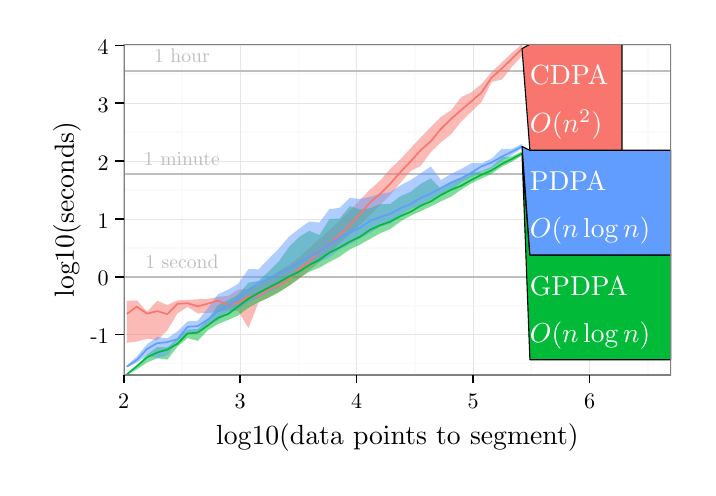
\begin{tikzpicture}[x=1pt,y=1pt]
\definecolor{fillColor}{RGB}{255,255,255}
\path[use as bounding box,fill=fillColor,fill opacity=0.00] (0,0) rectangle (238.49,158.99);
\begin{scope}
\path[clip] (  0.00,  0.00) rectangle (238.49,158.99);
\definecolor{drawColor}{RGB}{255,255,255}
\definecolor{fillColor}{RGB}{255,255,255}

\path[draw=drawColor,line width= 0.6pt,line join=round,line cap=round,fill=fillColor] (  0.00,  0.00) rectangle (238.49,158.99);
\end{scope}
\begin{scope}
\path[clip] ( 34.70, 33.48) rectangle (232.49,152.99);
\definecolor{fillColor}{RGB}{255,255,255}

\path[fill=fillColor] ( 34.70, 33.48) rectangle (232.49,152.99);
\definecolor{drawColor}{gray}{0.98}

\path[draw=drawColor,line width= 0.6pt,line join=round] ( 34.70, 37.63) --
	(232.49, 37.63);

\path[draw=drawColor,line width= 0.6pt,line join=round] ( 34.70, 58.53) --
	(232.49, 58.53);

\path[draw=drawColor,line width= 0.6pt,line join=round] ( 34.70, 79.43) --
	(232.49, 79.43);

\path[draw=drawColor,line width= 0.6pt,line join=round] ( 34.70,100.33) --
	(232.49,100.33);

\path[draw=drawColor,line width= 0.6pt,line join=round] ( 34.70,121.23) --
	(232.49,121.23);

\path[draw=drawColor,line width= 0.6pt,line join=round] ( 34.70,142.13) --
	(232.49,142.13);

\path[draw=drawColor,line width= 0.6pt,line join=round] ( 55.74, 33.48) --
	( 55.74,152.99);

\path[draw=drawColor,line width= 0.6pt,line join=round] ( 97.82, 33.48) --
	( 97.82,152.99);

\path[draw=drawColor,line width= 0.6pt,line join=round] (139.91, 33.48) --
	(139.91,152.99);

\path[draw=drawColor,line width= 0.6pt,line join=round] (181.99, 33.48) --
	(181.99,152.99);

\path[draw=drawColor,line width= 0.6pt,line join=round] (224.07, 33.48) --
	(224.07,152.99);
\definecolor{drawColor}{gray}{0.90}

\path[draw=drawColor,line width= 0.2pt,line join=round] ( 34.70, 48.08) --
	(232.49, 48.08);

\path[draw=drawColor,line width= 0.2pt,line join=round] ( 34.70, 68.98) --
	(232.49, 68.98);

\path[draw=drawColor,line width= 0.2pt,line join=round] ( 34.70, 89.88) --
	(232.49, 89.88);

\path[draw=drawColor,line width= 0.2pt,line join=round] ( 34.70,110.78) --
	(232.49,110.78);

\path[draw=drawColor,line width= 0.2pt,line join=round] ( 34.70,131.68) --
	(232.49,131.68);

\path[draw=drawColor,line width= 0.2pt,line join=round] ( 34.70,152.58) --
	(232.49,152.58);

\path[draw=drawColor,line width= 0.2pt,line join=round] ( 34.70, 33.48) --
	( 34.70,152.99);

\path[draw=drawColor,line width= 0.2pt,line join=round] ( 76.78, 33.48) --
	( 76.78,152.99);

\path[draw=drawColor,line width= 0.2pt,line join=round] (118.86, 33.48) --
	(118.86,152.99);

\path[draw=drawColor,line width= 0.2pt,line join=round] (160.95, 33.48) --
	(160.95,152.99);

\path[draw=drawColor,line width= 0.2pt,line join=round] (203.03, 33.48) --
	(203.03,152.99);
\definecolor{drawColor}{RGB}{190,190,190}

\path[draw=drawColor,line width= 0.6pt,line join=round] ( 34.70, 68.98) -- (232.49, 68.98);

\path[draw=drawColor,line width= 0.6pt,line join=round] ( 34.70,106.15) -- (232.49,106.15);

\path[draw=drawColor,line width= 0.6pt,line join=round] ( 34.70,143.31) -- (232.49,143.31);
\definecolor{fillColor}{RGB}{248,118,109}

\path[fill=fillColor,fill opacity=0.50] ( 35.81, 60.27) --
	( 39.47, 60.41) --
	( 43.14, 56.36) --
	( 46.80, 60.30) --
	( 50.46, 58.78) --
	( 54.12, 60.46) --
	( 57.79, 60.60) --
	( 61.45, 60.85) --
	( 65.11, 60.94) --
	( 68.77, 61.74) --
	( 72.43, 62.07) --
	( 76.10, 64.32) --
	( 79.76, 64.59) --
	( 83.42, 66.01) --
	( 87.08, 68.46) --
	( 90.74, 71.05) --
	( 94.41, 73.24) --
	( 98.07, 75.89) --
	(101.73, 79.27) --
	(105.39, 82.68) --
	(109.05, 85.88) --
	(112.72, 89.24) --
	(116.38, 92.77) --
	(120.04, 96.72) --
	(123.70,100.45) --
	(127.36,103.76) --
	(131.03,107.98) --
	(134.69,111.39) --
	(138.35,115.41) --
	(142.01,119.27) --
	(145.67,123.07) --
	(149.34,126.76) --
	(153.00,129.17) --
	(156.66,133.89) --
	(160.32,135.58) --
	(163.99,138.67) --
	(167.65,142.92) --
	(171.31,146.44) --
	(174.97,149.89) --
	(178.63,152.99) --
	(178.63,148.74) --
	(174.97,144.85) --
	(171.31,140.19) --
	(167.65,139.39) --
	(163.99,132.05) --
	(160.32,128.63) --
	(156.66,125.06) --
	(153.00,120.46) --
	(149.34,117.59) --
	(145.67,114.03) --
	(142.01,109.09) --
	(138.35,107.16) --
	(134.69,102.98) --
	(131.03, 98.57) --
	(127.36, 94.95) --
	(123.70, 91.35) --
	(120.04, 87.71) --
	(116.38, 84.32) --
	(112.72, 80.95) --
	(109.05, 77.70) --
	(105.39, 74.27) --
	(101.73, 71.22) --
	( 98.07, 68.16) --
	( 94.41, 65.64) --
	( 90.74, 63.56) --
	( 87.08, 61.39) --
	( 83.42, 59.71) --
	( 79.76, 50.40) --
	( 76.10, 56.58) --
	( 72.43, 56.93) --
	( 68.77, 56.18) --
	( 65.11, 55.92) --
	( 61.45, 55.76) --
	( 57.79, 58.06) --
	( 54.12, 55.76) --
	( 50.46, 49.59) --
	( 46.80, 46.06) --
	( 43.14, 46.61) --
	( 39.47, 45.59) --
	( 35.81, 45.10) --
	cycle;
\definecolor{fillColor}{RGB}{0,186,56}

\path[fill=fillColor,fill opacity=0.50] ( 35.81, 33.92) --
	( 39.47, 36.85) --
	( 43.14, 40.84) --
	( 46.80, 43.60) --
	( 50.46, 43.45) --
	( 54.12, 46.72) --
	( 57.79, 49.89) --
	( 61.45, 50.11) --
	( 65.11, 53.52) --
	( 68.77, 58.73) --
	( 72.43, 60.48) --
	( 76.10, 62.62) --
	( 79.76, 66.84) --
	( 83.42, 67.50) --
	( 87.08, 70.88) --
	( 90.74, 74.51) --
	( 94.41, 79.72) --
	( 98.07, 83.37) --
	(101.73, 85.57) --
	(105.39, 84.06) --
	(109.05, 89.85) --
	(112.72, 90.02) --
	(116.38, 94.51) --
	(120.04, 93.29) --
	(123.70, 93.73) --
	(127.36, 95.26) --
	(131.03, 95.28) --
	(134.69, 98.11) --
	(138.35, 99.66) --
	(142.01,102.55) --
	(145.67,104.57) --
	(149.34,100.67) --
	(153.00,103.01) --
	(156.66,104.80) --
	(160.32,106.57) --
	(163.99,107.14) --
	(167.65,108.75) --
	(171.31,112.11) --
	(174.97,112.51) --
	(178.63,114.26) --
	(178.63,112.81) --
	(174.97,110.53) --
	(171.31,108.75) --
	(167.65,106.19) --
	(163.99,104.49) --
	(160.32,102.75) --
	(156.66,100.52) --
	(153.00, 97.92) --
	(149.34, 96.23) --
	(145.67, 94.38) --
	(142.01, 92.70) --
	(138.35, 91.01) --
	(134.69, 88.97) --
	(131.03, 86.25) --
	(127.36, 84.67) --
	(123.70, 82.64) --
	(120.04, 80.59) --
	(116.38, 78.87) --
	(112.72, 76.25) --
	(109.05, 74.34) --
	(105.39, 72.25) --
	(101.73, 70.80) --
	( 98.07, 68.50) --
	( 94.41, 65.75) --
	( 90.74, 63.32) --
	( 87.08, 61.49) --
	( 83.42, 59.76) --
	( 79.76, 57.75) --
	( 76.10, 55.03) --
	( 72.43, 53.37) --
	( 68.77, 51.88) --
	( 65.11, 49.66) --
	( 61.45, 45.83) --
	( 57.79, 46.82) --
	( 54.12, 43.75) --
	( 50.46, 39.06) --
	( 46.80, 39.54) --
	( 43.14, 38.02) --
	( 39.47, 35.50) --
	( 35.81, 33.48) --
	cycle;
\definecolor{fillColor}{RGB}{97,156,255}

\path[fill=fillColor,fill opacity=0.50] ( 35.81, 36.85) --
	( 39.47, 40.21) --
	( 43.14, 44.58) --
	( 46.80, 47.23) --
	( 50.46, 46.72) --
	( 54.12, 49.27) --
	( 57.79, 52.85) --
	( 61.45, 53.11) --
	( 65.11, 57.59) --
	( 68.77, 62.66) --
	( 72.43, 64.32) --
	( 76.10, 66.44) --
	( 79.76, 71.75) --
	( 83.42, 71.67) --
	( 87.08, 75.45) --
	( 90.74, 79.18) --
	( 94.41, 83.46) --
	( 98.07, 86.32) --
	(101.73, 88.92) --
	(105.39, 88.58) --
	(109.05, 93.41) --
	(112.72, 93.88) --
	(116.38, 97.47) --
	(120.04, 97.12) --
	(123.70, 97.83) --
	(127.36, 98.98) --
	(131.03, 99.54) --
	(134.69,102.00) --
	(138.35,103.91) --
	(142.01,106.30) --
	(145.67,108.83) --
	(149.34,103.91) --
	(153.00,106.18) --
	(156.66,107.92) --
	(160.32,110.00) --
	(163.99,110.03) --
	(167.65,111.69) --
	(171.31,115.21) --
	(174.97,115.24) --
	(178.63,117.01) --
	(178.63,115.48) --
	(174.97,112.93) --
	(171.31,111.01) --
	(167.65,108.14) --
	(163.99,106.91) --
	(160.32,105.05) --
	(156.66,103.09) --
	(153.00,100.21) --
	(149.34, 98.37) --
	(145.67, 96.82) --
	(142.01, 94.83) --
	(138.35, 93.38) --
	(134.69, 91.15) --
	(131.03, 88.16) --
	(127.36, 87.10) --
	(123.70, 84.76) --
	(120.04, 82.79) --
	(116.38, 80.70) --
	(112.72, 78.91) --
	(109.05, 76.00) --
	(105.39, 74.32) --
	(101.73, 72.88) --
	( 98.07, 70.08) --
	( 94.41, 68.25) --
	( 90.74, 65.14) --
	( 87.08, 63.36) --
	( 83.42, 61.32) --
	( 79.76, 59.76) --
	( 76.10, 57.30) --
	( 72.43, 56.07) --
	( 68.77, 53.11) --
	( 65.11, 52.00) --
	( 61.45, 48.26) --
	( 57.79, 48.35) --
	( 54.12, 45.83) --
	( 50.46, 40.63) --
	( 46.80, 39.54) --
	( 43.14, 40.63) --
	( 39.47, 38.02) --
	( 35.81, 36.20) --
	cycle;
\definecolor{drawColor}{RGB}{248,118,109}

\path[draw=drawColor,line width= 0.6pt,line join=round] ( 35.81, 55.54) --
	( 39.47, 58.19) --
	( 43.14, 55.64) --
	( 46.80, 56.58) --
	( 50.46, 55.48) --
	( 54.12, 59.19) --
	( 57.79, 59.42) --
	( 61.45, 58.29) --
	( 65.11, 59.27) --
	( 68.77, 60.34) --
	( 72.43, 58.71) --
	( 76.10, 59.63) --
	( 79.76, 61.88) --
	( 83.42, 61.98) --
	( 87.08, 64.42) --
	( 90.74, 65.76) --
	( 94.41, 68.24) --
	( 98.07, 71.71) --
	(101.73, 74.39) --
	(105.39, 78.26) --
	(109.05, 81.00) --
	(112.72, 84.16) --
	(116.38, 87.61) --
	(120.04, 91.59) --
	(123.70, 95.87) --
	(127.36, 98.91) --
	(131.03,102.60) --
	(134.69,106.80) --
	(138.35,110.62) --
	(142.01,114.72) --
	(145.67,117.90) --
	(149.34,122.41) --
	(153.00,126.01) --
	(156.66,129.27) --
	(160.32,132.34) --
	(163.99,135.56) --
	(167.65,140.95) --
	(171.31,144.17) --
	(174.97,147.75) --
	(178.63,151.44);
\definecolor{drawColor}{RGB}{0,186,56}

\path[draw=drawColor,line width= 0.6pt,line join=round] ( 35.81, 33.70) --
	( 39.47, 36.69) --
	( 43.14, 39.88) --
	( 46.80, 41.61) --
	( 50.46, 42.66) --
	( 54.12, 44.78) --
	( 57.79, 48.48) --
	( 61.45, 48.82) --
	( 65.11, 51.39) --
	( 68.77, 54.15) --
	( 72.43, 55.51) --
	( 76.10, 58.29) --
	( 79.76, 61.02) --
	( 83.42, 63.14) --
	( 87.08, 65.05) --
	( 90.74, 66.96) --
	( 94.41, 69.05) --
	( 98.07, 70.84) --
	(101.73, 73.20) --
	(105.39, 75.13) --
	(109.05, 77.69) --
	(112.72, 79.55) --
	(116.38, 81.66) --
	(120.04, 83.42) --
	(123.70, 85.94) --
	(127.36, 87.60) --
	(131.03, 88.91) --
	(134.69, 90.87) --
	(138.35, 92.44) --
	(142.01, 94.64) --
	(145.67, 96.20) --
	(149.34, 98.50) --
	(153.00,100.40) --
	(156.66,101.87) --
	(160.32,103.97) --
	(163.99,105.84) --
	(167.65,107.41) --
	(171.31,109.74) --
	(174.97,111.53) --
	(178.63,113.49);
\definecolor{drawColor}{RGB}{97,156,255}

\path[draw=drawColor,line width= 0.6pt,line join=round] ( 35.81, 36.53) --
	( 39.47, 38.94) --
	( 43.14, 42.90) --
	( 46.80, 44.98) --
	( 50.46, 45.35) --
	( 54.12, 46.45) --
	( 57.79, 50.88) --
	( 61.45, 51.14) --
	( 65.11, 53.52) --
	( 68.77, 56.65) --
	( 72.43, 58.46) --
	( 76.10, 61.21) --
	( 79.76, 64.23) --
	( 83.42, 66.61) --
	( 87.08, 68.34) --
	( 90.74, 70.27) --
	( 94.41, 71.94) --
	( 98.07, 74.03) --
	(101.73, 76.17) --
	(105.39, 78.08) --
	(109.05, 80.86) --
	(112.72, 82.95) --
	(116.38, 85.03) --
	(120.04, 86.61) --
	(123.70, 89.13) --
	(127.36, 90.54) --
	(131.03, 91.73) --
	(134.69, 93.74) --
	(138.35, 95.19) --
	(142.01, 97.47) --
	(145.67, 99.04) --
	(149.34,101.05) --
	(153.00,103.03) --
	(156.66,104.57) --
	(160.32,106.58) --
	(163.99,108.91) --
	(167.65,110.25) --
	(171.31,112.37) --
	(174.97,114.16) --
	(178.63,116.05);
\definecolor{drawColor}{RGB}{190,190,190}

\node[text=drawColor,anchor=base,inner sep=0pt, outer sep=0pt, scale=  0.71] at ( 55.74, 71.92) {1 second};

\node[text=drawColor,anchor=base,inner sep=0pt, outer sep=0pt, scale=  0.71] at ( 55.74,109.08) {1 minute};

\node[text=drawColor,anchor=base,inner sep=0pt, outer sep=0pt, scale=  0.71] at ( 55.74,146.25) {1 hour};
\end{scope}
\begin{scope}
\path[clip] ( 34.70, 33.48) rectangle (232.49,152.99);
\definecolor{drawColor}{RGB}{0,0,0}
\definecolor{fillColor}{RGB}{0,186,56}

\path[draw=drawColor,line width= 0.4pt,line join=round,line cap=round,fill=fillColor] (178.63,113.49) --
	(181.48, 76.83) --
	(232.49, 76.83) --
	(232.49, 38.99) --
	(181.48, 38.99) --
	cycle;
\definecolor{fillColor}{RGB}{97,156,255}

\path[draw=drawColor,line width= 0.4pt,line join=round,line cap=round,fill=fillColor] (178.63,116.05) --
	(181.48,114.68) --
	(232.49,114.68) --
	(232.49, 76.83) --
	(181.48, 76.83) --
	cycle;
\definecolor{fillColor}{RGB}{248,118,109}

\path[draw=drawColor,line width= 0.4pt,line join=round,line cap=round,fill=fillColor] (178.63,151.44) --
	(181.48,152.99) --
	(214.75,152.99) --
	(214.75,114.68) --
	(181.48,114.68) --
	cycle;
\definecolor{drawColor}{RGB}{255,255,255}

\node[text=drawColor,anchor=base west,inner sep=0pt, outer sep=0pt, scale=  0.99] at (181.48, 62.36) {GPDPA};

\node[text=drawColor,anchor=base west,inner sep=0pt, outer sep=0pt, scale=  0.99] at (181.48, 45.29) {$O(n \log n)$};

\node[text=drawColor,anchor=base west,inner sep=0pt, outer sep=0pt, scale=  0.99] at (181.48,100.21) {PDPA};

\node[text=drawColor,anchor=base west,inner sep=0pt, outer sep=0pt, scale=  0.99] at (181.48, 83.14) {$O(n \log n)$};

\node[text=drawColor,anchor=base west,inner sep=0pt, outer sep=0pt, scale=  1.00] at (181.48,138.34) {CDPA};

\node[text=drawColor,anchor=base west,inner sep=0pt, outer sep=0pt, scale=  1.00] at (181.48,121.06) {$O(n^2)$};
\definecolor{drawColor}{gray}{0.50}

\path[draw=drawColor,line width= 0.6pt,line join=round,line cap=round] ( 34.70, 33.48) rectangle (232.49,152.99);
\end{scope}
\begin{scope}
\path[clip] (  0.00,  0.00) rectangle (238.49,158.99);
\definecolor{drawColor}{RGB}{0,0,0}

\node[text=drawColor,anchor=base east,inner sep=0pt, outer sep=0pt, scale=  0.80] at ( 29.30, 44.78) {-1};

\node[text=drawColor,anchor=base east,inner sep=0pt, outer sep=0pt, scale=  0.80] at ( 29.30, 65.68) {0};

\node[text=drawColor,anchor=base east,inner sep=0pt, outer sep=0pt, scale=  0.80] at ( 29.30, 86.58) {1};

\node[text=drawColor,anchor=base east,inner sep=0pt, outer sep=0pt, scale=  0.80] at ( 29.30,107.48) {2};

\node[text=drawColor,anchor=base east,inner sep=0pt, outer sep=0pt, scale=  0.80] at ( 29.30,128.38) {3};

\node[text=drawColor,anchor=base east,inner sep=0pt, outer sep=0pt, scale=  0.80] at ( 29.30,149.27) {4};
\end{scope}
\begin{scope}
\path[clip] (  0.00,  0.00) rectangle (238.49,158.99);
\definecolor{drawColor}{RGB}{0,0,0}

\path[draw=drawColor,line width= 0.6pt,line join=round] ( 31.70, 48.08) --
	( 34.70, 48.08);

\path[draw=drawColor,line width= 0.6pt,line join=round] ( 31.70, 68.98) --
	( 34.70, 68.98);

\path[draw=drawColor,line width= 0.6pt,line join=round] ( 31.70, 89.88) --
	( 34.70, 89.88);

\path[draw=drawColor,line width= 0.6pt,line join=round] ( 31.70,110.78) --
	( 34.70,110.78);

\path[draw=drawColor,line width= 0.6pt,line join=round] ( 31.70,131.68) --
	( 34.70,131.68);

\path[draw=drawColor,line width= 0.6pt,line join=round] ( 31.70,152.58) --
	( 34.70,152.58);
\end{scope}
\begin{scope}
\path[clip] (  0.00,  0.00) rectangle (238.49,158.99);
\definecolor{drawColor}{RGB}{0,0,0}

\path[draw=drawColor,line width= 0.6pt,line join=round] ( 34.70, 30.48) --
	( 34.70, 33.48);

\path[draw=drawColor,line width= 0.6pt,line join=round] ( 76.78, 30.48) --
	( 76.78, 33.48);

\path[draw=drawColor,line width= 0.6pt,line join=round] (118.86, 30.48) --
	(118.86, 33.48);

\path[draw=drawColor,line width= 0.6pt,line join=round] (160.95, 30.48) --
	(160.95, 33.48);

\path[draw=drawColor,line width= 0.6pt,line join=round] (203.03, 30.48) --
	(203.03, 33.48);
\end{scope}
\begin{scope}
\path[clip] (  0.00,  0.00) rectangle (238.49,158.99);
\definecolor{drawColor}{RGB}{0,0,0}

\node[text=drawColor,anchor=base,inner sep=0pt, outer sep=0pt, scale=  0.80] at ( 34.70, 21.46) {2};

\node[text=drawColor,anchor=base,inner sep=0pt, outer sep=0pt, scale=  0.80] at ( 76.78, 21.46) {3};

\node[text=drawColor,anchor=base,inner sep=0pt, outer sep=0pt, scale=  0.80] at (118.86, 21.46) {4};

\node[text=drawColor,anchor=base,inner sep=0pt, outer sep=0pt, scale=  0.80] at (160.95, 21.46) {5};

\node[text=drawColor,anchor=base,inner sep=0pt, outer sep=0pt, scale=  0.80] at (203.03, 21.46) {6};
\end{scope}
\begin{scope}
\path[clip] (  0.00,  0.00) rectangle (238.49,158.99);
\definecolor{drawColor}{RGB}{0,0,0}

\node[text=drawColor,anchor=base,inner sep=0pt, outer sep=0pt, scale=  1.00] at (133.59,  8.40) {log10(data points to segment)};
\end{scope}
\begin{scope}
\path[clip] (  0.00,  0.00) rectangle (238.49,158.99);
\definecolor{drawColor}{RGB}{0,0,0}

\node[text=drawColor,rotate= 90.00,anchor=base,inner sep=0pt, outer sep=0pt, scale=  1.00] at ( 16.66, 93.24) {log10(seconds)};
\end{scope}
\end{tikzpicture}
